% Chapter Template

\chapter{Literature Review} % Main chapter title
%\doublespacing
\label{Chapter2} % Change X to a consecutive number; for referencing this chapter elsewhere, use \ref{ChapterX}
\section{Molecular Simulations of Molecules Mimicking Asphaltenes}

Asphaltenes, unlike the majority of the compounds, are not defined on a molecular basis. The most accepted definition is that they are a fraction of crude oil insoluble in n-alkanes (pentane, hexane, and heptane) and soluble in toluene \cite{SJOBLOM2003399}. Due to uncertainties related to its structures, much work has been done to develop model compounds that have a well-defined structure and can represent asphaltenes. The two categories of models presented in the literature are the archipelago and continental models. In the archipelago model, asphaltenes consist of polyaromatic parts linked together by aliphatic or naphthenic moieties and, in the continental model, they consist of a single
polyaromatic ring with linked aliphatic or naphthenic chains \cite{doi:10.1021/ef900975e,doi:10.1080/0892702031000148762}. The choice of the model's structure, such as chemical bonding, is highly essential since some structures can cause the occurrence of high energies regions during the simulation \cite{doi:10.1021/ef200507c} .   

In order to evaluate the strengths and shortcomings of alphaltenes models, papers have been published about the calculations of various properties. There are some concordances in studies of theses models with molecular simulation, such as the influence of the model in the packing tendency of the molecule \cite{doi:10.1080/10298436.2011.575141}. \citeonline {doi:10.1021/ef9004576} utilized molecular dynamics in the study of the nanoaggregation of four types of model asphaltene molecules in binary mixtures of toluene and water. The authors observed that, in thin films of toluene trapped between two aqueous phases, both interface-bound and core-bound asphaltenes have similar diffusion behavior. \citeonline{doi:10.1021/acs.energyfuels.6b02161} reported molecular dynamics simulations of four model asphaltenes. They alleged that there is no formation of nanoaggregates, and that the distribution of asphaltene clusters is continuous for mixtures of asphaltene in heptane. 

Molecular dynamics simulations were also utilized in the study of \citeonline{ervik20162}  to obtain the correct interfacial orientation of asphaltenes using a coarse-grained model of the interface and a representative model for the asphaltene molecules. Also using a coarse-grained force field, \citeonline{doi:10.1021/ef502209j} carried molecular simulations with a continental asphaltene model. The results reproduced experimental data of the strong aggregation
of asphaltene molecules in n-heptane and high solubility in toluene. \citeonline{doi:10.1021/ef5020428} performed a molecular
dynamics study with the GROMOS 45a3 force field \cite{JCC:JCC1078} to identify the structural features of different asphaltene molecules.

\citeonline{doi:10.1021/ef301610q} employed the archipelago model in their work to investigate the interfacial behavior of asphaltene molecules at the oil-water interface using molecular dynamics simulations with the OPLS-AA force field \cite{doi:10.1021/ja00214a001}. They found that asphaltenes are preferably distributed in the oil phase in the case of pure toluene and at the oil-water interface
in the case of pure heptane. They also discovered an
oscillatory behavior of asphaltene molecules at the oil-water interface when using the archipelago model. \citeonline{doi:10.1021/jp407363p} used a perylene based model to study molecular association and interaction as well as the adsorption properties of the perylene molecule at the water/toluene or water/heptane interface. 

\section{Coarse-Grained (CG) Force Fields}


Molecular simulations can be carried out at different levels of description. The detailed atomistic level or \textit{ab initio} level is described by the laws of quantum mechanics. The system consists of a set of subatomic particles in which Schrodinger's equation is solved for all of them. The next level is the atomistic description. It considers that the system is made up of atoms following the laws of classical mechanics.  Force fields at this level are based on van der Waals interactions, which may include neutral or Coulombic charged sites. Contributions due to intramolecular interactions such as bond-stretching, angle-bending, and torsion are also usually accounted in these kinds of force fields. When the simulation scale needs to be increased, and the atomistic simulations become too computationally expensive such as in the study of biological systems, the coarse-grained (CG) description is more suited. It considers that the system is made up of pseudo-atoms or beads that contain multiple atoms or even an entire molecule. 

There is an evident loss of information in grouping atoms; hence it is necessary to assure that the process of eliminating unnecessary or unimportant information ('coarse-graining') does not affect the system's physical behavior. Ideally, coarse-grained models need to have representability, robustness, transferability, and computational efficiency. Representability means that you can use a model at a state point other than the one in which it was parameterized. The other characteristic, robustness, is related to the model's ability to enable reliable predictions for various structural, thermodynamic, or transport properties. Finally, a transferable model is one in which the representation of atomic or chemical moieties have the same behavior in different molecules- e. g., a pseudo-atom representing $CH_{2}$ should have the same properties both in an alkene molecule and in a polyethylene molecule     \cite{doi:10.1146/annurev-chembioeng-061312-103314}. To achieve the cited goals, coarse-grained force fields are usually developed by mapping the atomistic model to define the pseudo-atoms, which are generally formed by similar functional groups. 

The level of coarse-graining also needs to be established. \citeonline{hadley2012} affirm that six heavy atoms (non-hydrogen atoms) per bead are traditionally used in order to not lose valuable details and to maintain isotropic representations of the beads. After the mapping, CG force fields needs to be parametrized. There are two different approaches, bottom up and top down, to link the simulations on the coarse-grained scale to another scale (schematically represented in \figref{fig:multiscale}). The bottom-up approach uses information of a more detailed scale such as the quantum mechanics description or the atomistic description to obtain information necessary to the parametrization. This method highly depends on the more detailed model quality to succeed. Meanwhile, the top down methodology obtains parameters from larger scales, namely experimental thermodynamic properties or structure based properties. 

\begin{figure}[H]
	\raggedleft
	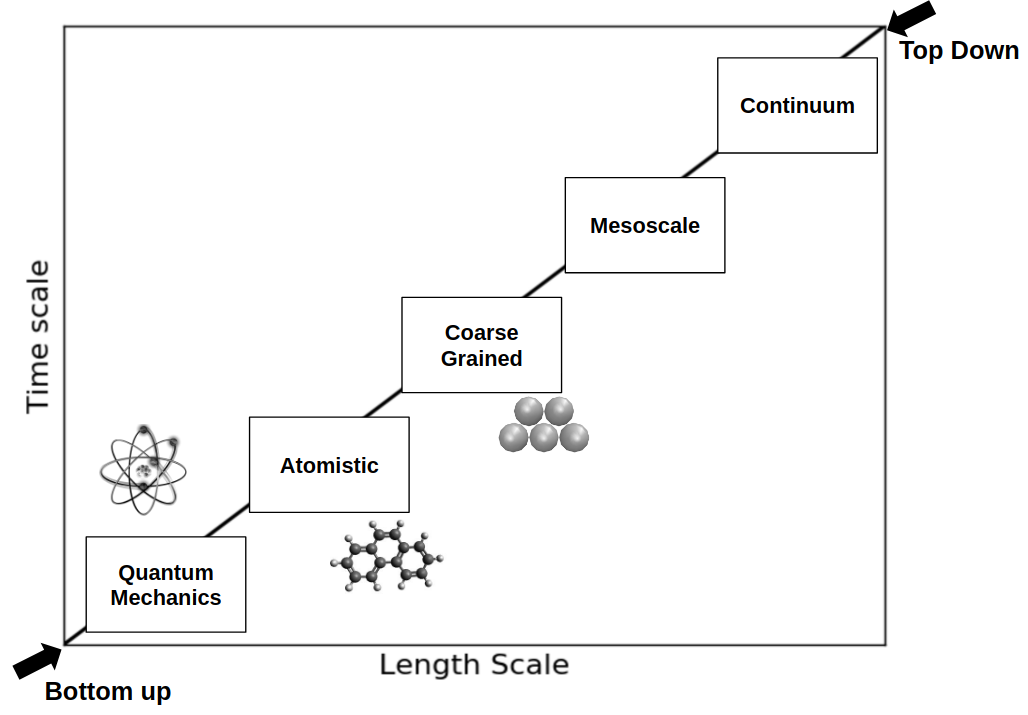
\includegraphics[width=0.9\textwidth]{Figures/multiscale}
	\caption{Schematic representation for the two different approaches of coarse-graining.}
	\label{fig:multiscale}
\end{figure}
\FloatBarrier

One of the first applications of coarse-grained models is in the study of protein folding \cite{levitt1975,levitt1976}. These earlier protein CG models were based on known molecular structure, and they contributed to the knowledge of physicochemical forces associated with protein folding and protein interactions \cite{koga2001}.  More recently, models focused on retaining the protein's chemical specificity. The Bereau and Deresmo model \cite{bereau2009} represents a single amino acid with a maximum of four beads, and it was used in studies of protein folding and aggregation. However, this model still needs tuning to improve protein stability \cite{bereau2010}. The OPEP (Optimized Potential for Efficient Protein Structure Prediction) model \cite{opep2014,opep2015} represents a single amino acid with a maximum of six beads. It was used to investigate a variety of phenomena, ranging from protein folding to the modeling of DNA-RNA complexes \cite{opep2011,opep2009,opep2014}. Other CG protein models used in the literature are the Scorpion (solvated coarse-grained protein interaction)  \cite{scorpion2013}, the UNRES (United Residue) \cite{unres2014} and the MARTINI model \cite{martini2013}. The latter one is the most popular model for CG modeling of membrane proteins \cite{martini20132}. The MARTINI force field is also extensively used as a CG model for water. This force field represents four water molecules as one bead using a shifted Lennard-Jones potential for non-bonded interactions. Despite its extensive use, the MARTINI water model does not properly reproduce properties such as interfacial tension and compressibility \cite{shinoda2010}. Besides, it can freeze at room temperature \cite{winger2009,martini2007}, which requires the use of anti-freeze agents during the simulations. This behavior can be explained by the high level of coarse-graining (4:1), the lack of explicit charges, and the use of a 12-6 potential. \citeonline{chiu2010} used the Morse Potential, which is softer than the LJ potential, to improve the MARTINI model. Meanwhile, \citeonline{shinoda2007} used different forms of the Mie potential to build a versatile and transferable coarse-grained model for surfactants/water systems using density, interfacial, and hydration free energies data. They selected a 12-4 Mie potential for water cross interactions and a 9-6 Mie potential for the surfactant (alkanes, oxyethylenes, ethylene glycols, ethers, and alcohols) interactions.

Outside of the Martini framework, \citeonline{10.1371/journal.pone.0028637} proposed the ELBA coarse-grained model for molecular dynamics simulations of lipids membranes. In this model, electrostatics are modeled explicitly by charges, and water molecules are represented by a single Lennard-Jones bead embedded with a point dipole. \citeonline{doi:10.1021/acs.jctc.5b00963} expanded the Elba force field to model 1-hexanol, 1-nonanol, n-hexane and n-nonane by representing three carbons with a single bead. Using different Mie and Morse potentials, \citeonline{shinoda2010} studied different levels of coarse-graining for water ranging from one to four molecules per bead. Other investigations also assessed the use of Soft-core potentials to study aqueous solutions of surfactants \cite{shinoda2007}, ionic liquids \cite{bhargava2009}, lipids \cite{shinoda20102}, and membranes \cite{pantano2009}. Another CG force field for water based on the Mie Potential is the SAFT-$\gamma$ Mie \cite{lobanova2015}. In this strategy, there are two different models: CGW1-vle and CGW1-ift. Both of them represent the water molecule as one bead, and the Mie Potential has a repulsive and attractive exponent equal to eight and six, respectively. The CGW1-vle model was parameterized using saturated-liquid density and vapor pressure data and should be used for simulations of aqueous systems in fluid-phase equilibrium at high temperatures and pressures. This model still suffers from premature freezing with a triple point at 343 K. The other model, CGW1-ift, was parameterized using saturated-liquid density and vapor-liquid interfacial tension. Hence, it is best suited for interfacial property calculations. Both models had temperature-dependent size and energy parameters and performed well for these properties over the entire liquid temperature range. The SAFT-$\gamma$ Mie force field has also been applied to other compounds with satisfactory results. \citeonline{muller2017} parameterized the force field for aromatic compounds and tested it with simulations of fluid phase equilibrium. \citeonline{herdes2015} carried out simulations of alkanes and light gases. \citeonline{lobanova2016} tested the force field with binary and ternary mixtures of water and carbon dioxide. There are also papers with the SAFT-$\gamma$ Mie about thermodynamic and transport properties of carbon dioxide and methane \cite{cassiano1,cassiano2} and water/oil interfacial tension \cite{herdes2017}.  

\section{Solvation Free Energies}

Solvation free energy calculations with molecular dynamics can be used to evaluate the quality of a coarse-grained force field, such as the ones described in the section above, since these estimations can reveal deficiencies in a force field. Besides this application, solvation free energies are used to obtain information about the behavior of the solvent in different chemical environments and to assess the influence of the solute's molecular geometry on the solvation phenomenon. Due to their range of application and inherent complexity, free energy calculations were the subject of a variety of studies in the last decade interested in improving free energy simulations and post-processing methods \cite{mbar,bareva,dexp,gdel}s.

Recent papers \cite{PMID:24928188,mobley2017} made available a big database of hydration free energy of small molecules using the GAFF force field. \citeonline{Beckstein2014} also calculated the hydration free energies for fifty two compounds with the OPLS-AA force field. They obtained an overall root mean square deviation to the experimental data of 1.75 kcal/mol and concluded that the reproducibility of the Lennard-Jones parameters is the main limiter of the precision of their results. \citeonline{izairi2017} also studied hydration free energies but with the intention of comparing the polar and nonpolar contributions. \citeauthor{garrido2011} (2009, 2011) calculated the free energy of solvation of large alkanes in 1-octanol and water with three different force fields (TraPPE, GROMOS, OPLS-AA/TraPPE) and the solvation free energy of propane and benzene in non aqueous solvents like n-hexadecane, n-hexane, ethylbenzene, and acetone  with the force fields TraPPE-UA and TraPPE-AA. \citeonline{roy2017} addressed the choice of the Lennard-Jones parameters for predicting solvation free energy in 1-octanol. They calculated the solvation free energy of a set of 205 small organic molecules in 1-octanol and found that the force field parametrization of n-octanol proposed by \citeonline{doi:10.1063/1.2972978} provided the best agreement. \citeonline{goncalves} calculated the free energy of solvation using the polarizable continuum model coupled to molecular dynamics computer simulation with the GROMOS force field. These calculations were done with a representative set of solutes and with the solvents tetrachloride, chloroform, and benzene. Using the GAFF and the polarizable AMOEBA force fields, \citeonline{mohamed2016} evaluated the solvation free energy of small molecules in toluene, chloroform, and acetonitrile, and obtained a mean unsigned error of 1.22 kcal/mol for AMOEBA and 0.66 kcal/mol for GAFF. To define the role of water as solvent in the docking structure determination of proteins, \citeonline{MATUBAYASI201745} developed a method to compute the solvation free energy of proteins while using OPLS-AA force field for the
solutes and TIP3P for water. \citeonline{doi:10.1021/acs.jctc.5b00963} expanded the Elba force field to calculate solvation free energies of more than 150 solutes taken from the Minnesota solvation
database in polar (water, hexanol, octanol and nonanol) and apolar (hexane,octane, and nonane) solvents. He obtained mean absolute deviations of 1 kcal/mol for water and 1.5 kcal/mol for hexane. In this model, three carbons are represented by a single bead and water is also represented by a single bead. 

Though this variety of data using the intramolecular Lennard-Jones potential, we are not aware of work using the Mie Potential in free energy calculations. We, in the present study, try to provide information about these predictions with the SAFT-$\gamma$ Mie coarse-grained force field.  As said before, the output of these calculations are highly dependent on the force field, and some coarse-grained models obtained satisfactory results for these kinds of simulations. Hence, knowing if other coarse-grained approaches have similar performances to the all-atoms force fields can help increase the scale of solvation free energy calculations. 

\section{Solvation Free Energy Calculation Methods}\label{SFECM}

Solvation free energy calculations account for the difference in free energy related to transferring the solute form ideal gas condition to the liquid solvent condition. To do that, we gradually insert the solute in the solvent. This process is mathematically carried out by using a coupling parameter ($\lambda$) on the total potential energy function, where $\lambda s$ represent the intermediate states in the transition from the ideal gal condition to the solvent condition. Hence,  during the solvation free energy simulations, we obtain total potential energies correspondent to these coupling parameters [($U(\lambda)$]. After the simulations, these potential energies need to be post-processed and analyzed to calculate the solvation free energies effectively. Since these calculations can have slow convergences, a lot of papers in the last decades focused on developing analysis methods to calculate free energies. Almost all methods rely on o the following approaches:  free energy perturbation (FEP) based methods, thermodynamic integration, and histograms.

\subsection{Thermodynamic integration}

The thermodynamic integration method \cite{kirkwood1935} uses equilibrium averages to evaluate the energy derivative with respect to the coupling parameter ($\lambda$): 
%Then, the free energies are calculated by  doing the derivative ($\frac{\partial G}{\partial \lambda} $):
%
%\begin{equation}
%\label{eq:ti1}
%\begin{aligned}
%\frac{\partial \beta G}{\partial \lambda} = - \frac{1}{Z (\lambda)}\frac{\partial Z}{\partial \lambda}
%\end{aligned}
%\end{equation}
%
%The Eq. \eqref{eq:dif} can be rewritten according to the Halmitonian of the system ($\mathcal{H}$):
%
%\begin{equation}
%\label{eq:ti2}
%\begin{aligned}
%\Delta G = - \kappa_{b}T ln \left( \frac{Z_{1}}{Z_{0}}\right) = -\kappa_{b}T ln \int \frac{exp(-\beta \mathcal{H} _{1}(r,p)) dr dp}{exp(-\beta \mathcal{H} _{0}(r,p)) dr dp}
%\end{aligned}
%\end{equation}

%Substituting Eq. \eqref{eq:ti2} in \eqref{eq:ti2} and adding the coupling parameter to the Halmitonian ($\mathcal{H} (r,p,\lambda)$) in order to describe the transition between the end states:

%\begin{equation}
%\label{eq:ti3}
%\begin{aligned}
%\frac{\partial \beta G}{\partial \lambda} =  \int \frac{\frac{\partial \mathcal{H} (r,p,\lambda)}{\partial \lambda}exp(-\beta \mathcal{H}(r,p,\lambda)) dr dp}{exp(-\beta \mathcal{H}(r,p,\lambda)) dr dp} =  \left \langle \frac{\partial \mathcal{H}(r,p,\lambda)}{\partial \lambda} \right \rangle 
%\end{aligned}
%\end{equation}

\begin{equation}
\label{eq:ti3}
\begin{aligned}
\frac{\partial (G \, 1/\kappa_{b}T) }{\partial \lambda} =  \left \langle \frac{\partial \mathcal{H}}{\partial \lambda} \right \rangle _{N,P,T} .
\end{aligned}
\end{equation}

In Eq. \eqref{eq:ti3}, $\kappa_{b}$ is the Boltzmann constant, $G$ is the Gibbs free energy and $\mathcal{H}$ is the Halmitonian of the system. The derivative is obtained for every configuration data between the states from simulations through an analytical expression. Some examples of methods for obtaining theses expressions are the trapezoidal rule or natural cubic spline \cite{bareva}. There are also more complex schemes that are usually system specific, such as as those found  in \citeonline{garrido2010} and \citeonline{shyu2009}. MD simulations for each coupling parameter $\lambda_{k}$ are carried out and the average over the derivative at each state is compute in order to obtain the final solvation free energy:

\begin{equation}
\label{eq:ti4}
\begin{aligned}
\Delta G \approx \int _{0}^{1}  \left \langle \frac{\partial \mathcal{H}}{\partial \lambda _{k}}  \right \rangle d \lambda .
\end{aligned}
\end{equation}

\subsection{Histograms}
%97
Histograms are used to compute probability distributions. Usually, every histogram count is treated as the number of visits to a specific state. The standard practice when using histograms is to use the weighted histogram analysis method (WHAM) developed by \citeonline{PhysRevLett.63.1195} and generalized by \citeonline{wham} \cite{freeenergy}. It puts together different histograms by minimizing the statistical error in the computed density of states and entropy function. This method describes the total probability distribution as a weighted unbiased sum of probability distributions from biased simulations. This method was developed to avoid problems related to data loss, high uncertainties, and the calculation of the constant added by the use of a biased potential \cite{ROUX1995275}. The probability distribution dependent on the potential energy ($U$) and temperature (T)  for the WHAM is

\begin{equation}
\label{eq:wham1}
\begin{aligned}
\tilde{\varrho_{r}^{*}}(U,T)  {}=& \frac{\sum_{i} f_{i}(U) \exp(- \beta U)}{\sum_{i} f_{tot,i} \exp(\beta _{i} \tilde{A}_{i} -\beta _{i} U) }, \\
& \exp(- \beta _{i} \tilde{A}_{i})  = \sum_{U} \tilde{\varrho_{r}^{*}}(U,T), \, and \\
& \tilde{\varrho_{r}}(U,T) = \frac{\tilde{\varrho_{r}^{*}}(U,T)}{\sum_{U} \tilde{\varrho_{r}^{*}}(U,T)},
\end{aligned}
\end{equation}
where $\beta = 1/\kappa_{b}T$, $\tilde{A}_{i}$ gives the free energy for run i, $f_{i}(U)$ is the number of counts of energy U for run i and $f_{tot,i}$ is the total number of counts in run i. Eq. \eqref{eq:wham1} is solved self consistently with the initial value for $\tilde{A}_{i}$ equals to zero. The final unnormalized probability distribution is then given by $\tilde{\varrho_{r}}(U,T)$.

\subsection{Free Energy Perturbation (FEP)}
%38
The free energy perturbation method \cite{zwanzig1954} is the oldest and one of the most general-purpose strategies to calculate free energy differences. In this method, the thermodynamics of two different systems (A and B) are related to the intention of evaluating differences in intermolecular potentials. This energy change from state A to state B is calculated by  

\begin{equation}
\label{eq:fep}
\begin{aligned}
\Delta G_{AB} = -\kappa_{b}T ln \langle{e^{-\beta (U_{B}-U_{A})}}\rangle_{A} .
\end{aligned}
\end{equation}

According to the equation above, the free energy difference is calculated by doing an average over the configurations of state A and B obtained during the simulation of state A. This method requires a great overlap between states (the state B needs to represent a small perturbation in state A) in order to obtain a rapid convergence of the free energy difference. To ensure overlap, it is possible to carry out simulations in N intermediate states between A and B, so Eq. \eqref{eq:fep} becomes:

\begin{equation}
\label{eq:fepint}
\begin{aligned}
\Delta G_{AB} = -\kappa_{b}T  \sum_{i=0}^{N}
ln \langle {e^{-\beta (U_{i+1}-U_{i})}} \rangle_{i} .
\end{aligned}
\end{equation}

This way of calculation $\Delta G$ in Eq. \ref{eq:fepint} is also called Exponential Averaging (EXP) \cite{zwanzig1955,bareva}. The direction of the transformation is crucial in this method. If the direction is of decreasing entropy, the step is of insertion ($\Delta G_{AB}$), and the method is called insertion exponential averaging (IEXP). When the direction is of increasing entropy, the step is of deletion ($\Delta G_{BA}$), and the method is labeled as deletion exponential averaging (DEXP). These directions can yield different values of free energy differences due to undersampling in the tail regions of the $\Delta G_{AB}$ distribution \cite{klimovich,pohorille2010}. These problems make the EXP methods not suited to calculate free energy differences when the system does not have sufficient overlap. For these cases, the Bennet Acceptance Ratio or the Multi-State Bennett Acceptance Ratio is more adequate.   

\subsubsection{Bennett Acceptance Ratio (BAR)}

The BAR method \cite{bennet1976} was developed with the intent of eliminating the direction bias in the free energy estimation with FEP. It uses the uncorrelated samples of the potential energy in both directions ($A \rightarrow B$ and $B \rightarrow A$) to obtain the free energy differences using the information in a statically optimal way. The free energy difference between two intermediate states is obtained using the potential energy difference ($\Delta U$) between states i and j. The calculation is done by solving self-consistently the following equations: 

\begin{equation}
\label{eq:bar1}
\begin{aligned}
\Delta G_{ij} = \frac{1}{\beta} ln \left( \dfrac{\sum_{k=1}^{N_{j}} \dfrac{1}{1+\exp[-\beta(\Delta U_{k}^{j}+C)]}}{\sum_{l=1}^{N_{i}} \dfrac{1}{1+\exp[-\beta(\Delta U_{l}^{i}-C)]}}\right) + C - \frac{1}{\beta}ln\left(\frac{N_{j}}{N_{i}}\right),
\end{aligned}
\end{equation}

\begin{equation}
\label{eq:bar2}
\begin{aligned}
C = \Delta G_{ij} + \frac{1}{\beta}ln\left(\frac{N_{j}}{N_{i}}\right).
\end{aligned}
\end{equation}

The total free energy difference between the end states is then given by the sum over differences of consecutive intermediate states. This method also provides a function to obtain the variance for the free energy differences, which is a minimum. The variance equation for any value of C is given by:

\begin{equation}
\label{eq:barvar}
\begin{aligned}
s_{ij}^{2} = \frac{1}{\beta^{2} N_{i}} \left[\dfrac{\langle{f^{2}(x)}\rangle_{i}}{\langle{f(x)}\rangle^{2}_{i}} - 1\right] + \frac{1}{\beta^{2} N_{j}} \left[\dfrac{\langle{f^{2}(x)}\rangle_{j}}{\langle{f(x)}\rangle^{2}_{j}} - 1\right],
\end{aligned}
\end{equation}
where $f(x)=1/(1+x)$ is the Fermi function and $x=\exp[\beta(\Delta U - C)]$. The variance of the free energy difference between end states can be calculated by assuming independent errors and summing over the variances of consecutive intermediate states. However, this assumption is not correct and there is no general formula to obtain a statistically unbiased estimate of an entire transformation with the BAR method \cite{bareva}. 

There are two other methods related to the BAR method that do not solve Eqs. \eqref{eq:bar1} and \eqref{eq:bar2} self consistently. By doing that, free energy differences will not have minimum variance, and the averages of Eqs. \eqref{eq:bar1} - \eqref{eq:barvar} are accumulated \cite{bareva}. The two methods are the Unoptimized Bennett Acceptance Ratio (UBAR) and the Range-Based Bennett Acceptance Ratio (RBAR). The first one avoids the self consistent solution of the BAR equations by defining $C=\beta^{-1}ln(N_{j}/N_{i})$. The UBAR method will be close to optimal when each intermediate free energy is relatively near zero. In turn, the RBAR method selects a range of initial guesses of the constant $C$ to calculate a range of $\Delta G_{ij}$. The value of free energy difference correspondent to the minimum variance is then used as input in Eq. \eqref{eq:bar2} to calculate the value of $C$. Hence, this method requires a good estimation of the initial range of the values of $C$. The RBAR can be advantageous when compared to BAR since only the accumulated averages need to be retained for postprocessing \cite{bareva}.  

\subsubsection{Multistate Bennet Acceptance Ratio (MBAR)}

The MBAR method \cite{mbar} is a further development of the BAR method, and is the one chosen to estimate the solvation free energies in this dissertation. This method consists of an estimator that computes free energies and their uncertainties of each $K$ state by minimizing the $K \times K$ matrix of variances simultaneously. The estimator solves the following equation for each $G_{i}$ self consistently:


\begin{equation}
\label{eq:mbar}
\begin{aligned}
G_{i} = \frac{1}{\beta}ln \sum_{k=1}^{K} \sum_{n=1}^{N_{k}}
\dfrac{\exp[-\beta U_{i}(x_{kn})]}{\sum_{l=1}^{K} N_{l} \exp[\beta (G_{l} - U_{l}(x_{kn}))]} .
\end{aligned}
\end{equation}

The equation above requires the evaluation of the potential energy $[U_{i}(x_{kn})]$ of  the $n_{th}$ uncorrelated configuration obtained at state K and  all uncorrelated configuration snapshots ($N_{k}$) from state $K$. Free energy changes between states are given then by $\Delta G_{ij} = G_{j} -  G_{i}$. The uncertainties  can be computed by :

\begin{equation}
\begin{aligned}
\delta _{ij}^{2} s_{ij} = s_{ii}^{2} + s_{jj}^{2} - 2 s_{ij}.
\end{aligned}
\end{equation}
where $s_{ij}$ is te covariance matrix. A further development of this method is available in Section \ref{mbar}.

